\minpurp{Selection-Sort}
Suche Minimum; Tausche es mit dem ersten Element; Wiederhole im Array [2...n], \textbf{ O\{$n^2$\}}

\minpurp{Bubble-Sort}
durchlaufe alle elemente und tausche element mit nachfolger wenn es kleiner ist als dieser; wiederhole bis das array sortiert ist. \textbf{O\{$n^2$\}}

\minpurp{Quicksort}
\halfpage{\begin{enumerate}
\item Wähle Pivot= letztes Element
\item lasse zeiger von beiden Enden des Restarrays nach innen laufen: \\
 wenn der rechte zeiger auf ein kleineres bzw. der linke auf ein größeres Element als das Pivot zeigt stoppe den zeiger; wenn beide stoppen tausche sie, wenn sich die Zeiger treffen tausche das Pivot nach innen 
\item Wiederhole Quicksort im Rechten und linken Teilarray.
\end{enumerate}
}
Laufzeit: best Case:$O(n\log_2n)$, worst-Case $O(n^2)$

\textbf{probabilistisch:} start: wähle zufälliges Element als Pivot und tausche ans ende, rest identisch

\quarterpage{
\minpurp{Heapsort}
Interpretation Array als binärer Heap;\\
a[2i] und a[2i+1] sind die Kinder von a[i] => Array durchläuft die Ebenen von oben nach unten, von rechts nach links

Heapbedingung: Knoten ist $\leq$ seine Kinder
}
\quarterpage{
z.B. $[\underbrace{37}, \underbrace{45,57}, \underbrace{59,58, 99}] $=\\
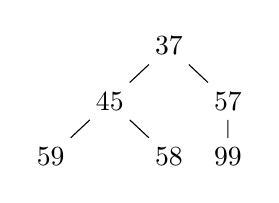
\begin{tikzpicture}[level distance=2em]
\node{37} 
child{ node{45}
child{ node{59}}
child{ node{58}}}
child{ node{57}
child{ node{99}}
}
;
\end{tikzpicture}
}

\minmeth{Einsickern}
Knoten verletzt die Heapbedingung: Tausche mit Kleinerem nachfolger; ggf. wiederholen

\minmeth{Downheap Revisited}
Folge dem Pfad der kleineren Nachfolger bis zum Blatt und speichere dessen index.\\ 
Vorgänger eines Blattes $b_i$ ist $\lfloor b_i /2 \rfloor $ => index des i. Knotens sind die vordersten i Bits des Blattindex

\textbf{Lineare Suche:}
Suche vom Pfadende aus die Stelle, an der die Wurzel eingefügt werden muss, schiebe alle Knoten um 1 Nach oben vom nachfolger der Wurzel angefangen.

\textbf{binärsuche:} analog zu lineare Suche nur mit binärer Suche 


\minmeth{Aufbau des Heaps}
Führe Einsichern für die Teilbäume durch (von unten rechts zur wurzel); \textbf{O(n)}

\minmeth{Heapsort}
Erzeuge Heap; 
Tausche das letzte Element mit dem ersten, Wurzel einsickern in [1...n-1] , wiederhole bis array leer; 
Laufzeit worst-case: $O(n\log_2n)$

\minpurp{Suche im Array}
\minmeth{Sequentiell}
gehe der reihe nach alle elemente durch bis das element gefunden \textbf{O(n)}

\minmeth{Binär}
Vorraussetzung: Sortiertes Array;
Wähle das mittlere Element; ist es kleiner als das zu suchende Wiederhole im linken Teilarray, analog bei größer\\
worst-Case: $O(\log_2n)$

\minmeth{Quick-Select}
ist das k. kleinste element gesucht. Analog zu probab. Quicksort, es muss allerdings immer nur das Teilarray sortiert werden, in den der k. Index fällt; durchschnitt \textbf{O(n)}